\documentclass[border=0.1cm, 12pt]{standalone}
\usepackage[utf8]{inputenc}

\usepackage{tikz}
\usepackage{amsfonts}
\usepackage{amsmath,amssymb}
\usepackage{systeme,mathtools}
\usetikzlibrary{positioning,arrows.meta,quotes}
\usetikzlibrary{shapes,snakes}
\usetikzlibrary{bayesnet}
\tikzset{>=latex}

\begin{document}
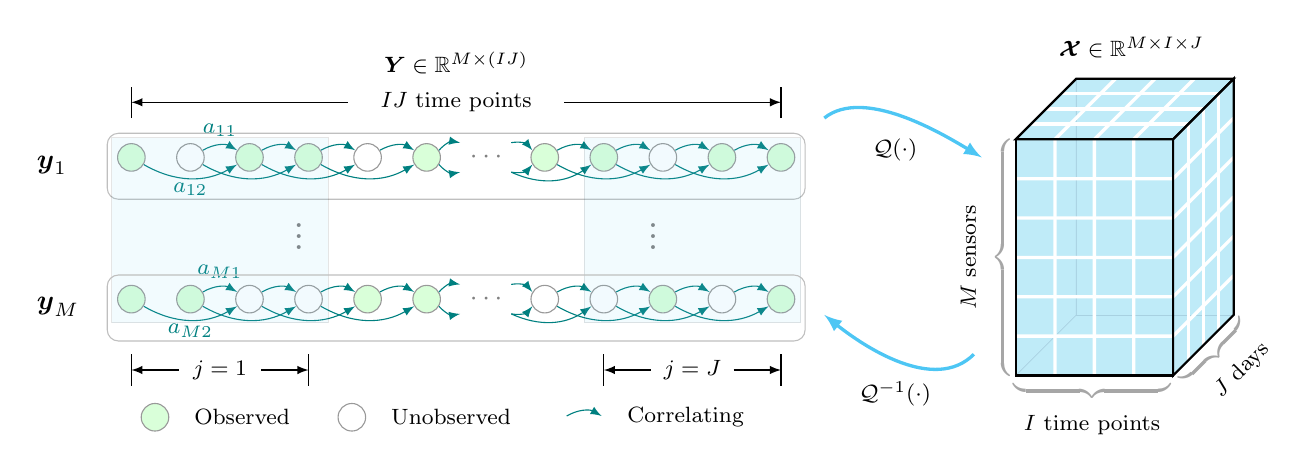
\begin{tikzpicture}

\node[circle,draw=gray!80,fill=green!15,inner sep=0pt,minimum size=0.35cm] (obs1) at (0-12,1.5) {};
\node[circle,draw=gray!80,fill=white,inner sep=0pt,minimum size=0.35cm] (obs11) at (0.75-12,1.5) {};
\node[circle,draw=gray!80,fill=green!15,inner sep=0pt,minimum size=0.35cm] (obs2) at (1.5-12,1.5) {};
\node[circle,draw=gray!80,fill=green!15,inner sep=0pt,minimum size=0.35cm] (obs22) at (2.25-12,1.5) {};
\node[circle,draw=gray!80,fill=white,inner sep=0pt,minimum size=0.35cm] (obs3) at (3-12,1.5) {};
\node[circle,draw=gray!80,fill=green!15,inner sep=0pt,minimum size=0.35cm] (obs33) at (3.75-12,1.5) {};
\node[text width=0.4cm] (obs4) at (4.5-12,1.5) {\color{gray}{$\LARGE{\cdots}$}};

\node[circle,draw=gray!80,fill=green!15,inner sep=0pt,minimum size=0.35cm] (obs44) at (5.25-12,1.5) {};
\node[circle,draw=gray!80,fill=green!15,inner sep=0pt,minimum size=0.35cm] (obs5) at (6-12,1.5) {};
\node[circle,draw=gray!80,fill=white,inner sep=0pt,minimum size=0.35cm] (obs55) at (6.75-12,1.5) {};
\node[circle,draw=gray!80,fill=green!15,inner sep=0pt,minimum size=0.35cm] (obs6) at (7.5-12,1.5) {};
\node[circle,draw=gray!80,fill=green!15,inner sep=0pt,minimum size=0.35cm] (obs66) at (8.25-12,1.5) {};

\path [draw,->,color=blue!50!green] (obs11) edge [bend left] node [right] {} (obs2);
\node[color = blue!50!green] () at (1.125-12, 1.85) {\footnotesize $a_{11}$};
\path [draw,->,color=blue!50!green] (obs2) edge [bend left] node [right] {} (obs22);
% \node[color = blue!50!green] () at (1.875-12, 1.85) {\footnotesize $a_{11}$};
\path [draw,->,color=blue!50!green] (obs22) edge [bend left] node [right] {} (obs3);
% \node[color = blue!50!green] () at (2.625-12, 1.85) {\footnotesize $a_{11}$};
\path [draw,->,color=blue!50!green] (obs3) edge [bend left] node [right] {} (obs33);
% \node[color = blue!50!green] () at (3.375-12, 1.85) {\footnotesize $a_{11}$};
\path [draw,->,color=blue!50!green] (obs33) edge [bend left] node [right] {} (obs4);
\path [draw,->,color=blue!50!green] (obs4) edge [bend left] node [right] {} (obs44);
% \node[color = blue!50!green] () at (5.625-12, 1.85) {\footnotesize $a_{11}$};
\path [draw,->,color=blue!50!green] (obs44) edge [bend left] node [right] {} (obs5);
% \node[color = blue!50!green] () at (6.375-12, 1.85) {\footnotesize $a_{11}$};
\path [draw,->,color=blue!50!green] (obs5) edge [bend left] node [right] {} (obs55);
% \node[color = blue!50!green] () at (7.125-12, 1.85) {\footnotesize $a_{11}$};
\path [draw,->,color=blue!50!green] (obs55) edge [bend left] node [right] {} (obs6);
% \node[color = blue!50!green] () at (7.875-12, 1.85) {\footnotesize $a_{11}$};
\path [draw,->,color=blue!50!green] (obs6) edge [bend left] node [right] {} (obs66);

\path [draw,->,color=blue!50!green] (obs1) edge [bend right] node [left] {} (obs2);
\node[color = blue!50!green] () at (0.75-12, 1.1) {\footnotesize $a_{12}$};
\path [draw,->,color=blue!50!green] (obs11) edge [bend right] node [left] {} (obs22);
% \node[color = blue!50!green] () at (1.5-12, 1.1) {\footnotesize $a_{12}$};
\path [draw,->,color=blue!50!green] (obs2) edge [bend right] node [left] {} (obs3);
% \node[color = blue!50!green] () at (2.25-12, 1.1) {\footnotesize $a_{12}$};
\path [draw,->,color=blue!50!green] (obs22) edge [bend right] node [left] {} (obs33);
% \node[color = blue!50!green] () at (3-12, 1.1) {\footnotesize $a_{12}$};
\path [draw,->,color=blue!50!green] (obs33) edge [bend right] node [left] {} (obs4);
\path [draw,->,color=blue!50!green] (obs4) edge [bend right] node [left] {} (obs44);
\path [draw,->,color=blue!50!green] (obs4) edge [bend right] node [left] {} (obs5);
% \node[color = blue!50!green] () at (5.25-12, 1.1) {\footnotesize $a_{12}$};
\path [draw,->,color=blue!50!green] (obs44) edge [bend right] node [left] {} (obs55);
% \node[color = blue!50!green] () at (6-12, 1.1) {\footnotesize $a_{12}$};
\path [draw,->,color=blue!50!green] (obs5) edge [bend right] node [left] {} (obs6);
% \node[color = blue!50!green] () at (6.75-12, 1.1) {\footnotesize $a_{12}$};
\path [draw,->,color=blue!50!green] (obs55) edge [bend right] node [left] {} (obs66);
% \node[color = blue!50!green] () at (7.5-12, 1.1) {\footnotesize $a_{12}$};


\plate[draw=gray!50] {}{(obs1)(obs66)}{};

\node[text width=0.4cm] (obs8) at (2.25-12,0.6) {\color{gray}{$\LARGE{\vdots}$}};
\node[text width=0.4cm] (obs8) at (-1-12,1.4) {\color{black}{${\boldsymbol{y}_{1}}$}};
\node[text width=0.4cm] (obs8) at (6.75-12,0.6) {\color{gray}{$\LARGE{\vdots}$}};
\node[text width=0.4cm] (obs8) at (-1-12,-0.4) {\color{black}{${\boldsymbol{y}_{M}}$}};

\node[circle,draw=gray!80,fill=green!15,inner sep=0pt,minimum size=0.35cm] (obs1) at (0-12,-0.3) {};
\node[color = blue!50!green] () at (1.125-12, 0.05) {\footnotesize $a_{M1}$};
\node[circle,draw=gray!80,fill=green!15,inner sep=0pt,minimum size=0.35cm] (obs11) at (0.75-12,-0.3) {};
% \node[color = blue!50!green] () at (1.875-12, 0.05) {\footnotesize $a_{M1}$};
\node[circle,draw=gray!80,fill=white,inner sep=0pt,minimum size=0.35cm] (obs2) at (1.5-12,-0.3) {};
% \node[color = blue!50!green] () at (2.625-12, 0.05) {\footnotesize $a_{M1}$};
\node[circle,draw=gray!80,fill=white,inner sep=0pt,minimum size=0.35cm] (obs22) at (2.25-12,-0.3) {};
% \node[color = blue!50!green] () at (3.375-12, 0.05) {\footnotesize $a_{M1}$};
\node[circle,draw=gray!80,fill=green!15,inner sep=0pt,minimum size=0.35cm] (obs3) at (3-12,-0.3) {};
\node[circle,draw=gray!80,fill=green!15,inner sep=0pt,minimum size=0.35cm] (obs33) at (3.75-12,-0.3) {};
\node[text width=0.4cm] (obs4) at (4.5-12,-0.3) {\color{gray}{$\LARGE{\cdots}$}};

\node[circle,draw=gray!80,fill=white,inner sep=0pt,minimum size=0.35cm] (obs44) at (5.25-12,-0.3) {};
% \node[color = blue!50!green] () at (5.625-12, 0.05) {\footnotesize $a_{M1}$};
\node[circle,draw=gray!80,fill=white,inner sep=0pt,minimum size=0.35cm] (obs5) at (6-12,-0.3) {};
% \node[color = blue!50!green] () at (6.375-12, 0.05) {\footnotesize $a_{M1}$};
\node[circle,draw=gray!80,fill=green!15,inner sep=0pt,minimum size=0.35cm] (obs55) at (6.75-12,-0.3) {};
% \node[color = blue!50!green] () at (7.125-12, 0.05) {\footnotesize $a_{M1}$};
\node[circle,draw=gray!80,fill=white,inner sep=0pt,minimum size=0.35cm] (obs6) at (7.5-12,-0.3) {};
% \node[color = blue!50!green] () at (7.875-12, 0.05) {\footnotesize $a_{M1}$};
\node[circle,draw=gray!80,fill=green!15,inner sep=0pt,minimum size=0.35cm] (obs66) at (8.25-12,-0.3) {};

\path [draw,->,color=blue!50!green] (obs1) edge [bend right] node [left] {} (obs2);
\node[color = blue!50!green] () at (0.75-12, -0.7) {\footnotesize $a_{M2}$};
\path [draw,->,color=blue!50!green] (obs11) edge [bend right] node [left] {} (obs22);
% \node[color = blue!50!green] () at (1.5-12, -0.7) {\footnotesize $a_{M2}$};
\path [draw,->,color=blue!50!green] (obs2) edge [bend right] node [left] {} (obs3);
% \node[color = blue!50!green] () at (2.25-12, -0.7) {\footnotesize $a_{M2}$};
\path [draw,->,color=blue!50!green] (obs22) edge [bend right] node [left] {} (obs33);
% \node[color = blue!50!green] () at (3-12, -0.7) {\footnotesize $a_{M2}$};
\path [draw,->,color=blue!50!green] (obs33) edge [bend right] node [left] {} (obs4);
\path [draw,->,color=blue!50!green] (obs4) edge [bend right] node [left] {} (obs44);
\path [draw,->,color=blue!50!green] (obs4) edge [bend right] node [left] {} (obs5);
% \node[color = blue!50!green] () at (5.25-12, -0.7) {\footnotesize $a_{M2}$};
\path [draw,->,color=blue!50!green] (obs44) edge [bend right] node [left] {} (obs55);
% \node[color = blue!50!green] () at (6-12, -0.7) {\footnotesize $a_{M2}$};
\path [draw,->,color=blue!50!green] (obs5) edge [bend right] node [left] {} (obs6);
% \node[color = blue!50!green] () at (6.75-12, -0.7) {\footnotesize $a_{M2}$};
\path [draw,->,color=blue!50!green] (obs55) edge [bend right] node [left] {} (obs66);
% \node[color = blue!50!green] () at (7.5-12, -0.7) {\footnotesize $a_{M2}$};


\path [draw,->,color=blue!50!green] (obs11) edge [bend left] node [right] {} (obs2);
\path [draw,->,color=blue!50!green] (obs2) edge [bend left] node [right] {} (obs22);
\path [draw,->,color=blue!50!green] (obs22) edge [bend left] node [right] {} (obs3);
\path [draw,->,color=blue!50!green] (obs3) edge [bend left] node [right] {} (obs33);
\path [draw,->,color=blue!50!green] (obs33) edge [bend left] node [right] {} (obs4);
\path [draw,->,color=blue!50!green] (obs4) edge [bend left] node [right] {} (obs44);
\path [draw,->,color=blue!50!green] (obs44) edge [bend left] node [right] {} (obs5);
\path [draw,->,color=blue!50!green] (obs5) edge [bend left] node [right] {} (obs55);
\path [draw,->,color=blue!50!green] (obs55) edge [bend left] node [right] {} (obs6);
\path [draw,->,color=blue!50!green] (obs6) edge [bend left] node [right] {} (obs66);
% \path [draw,->,color=red!50!gray] (obs66) edge [bend left] node [right] {} (obs7);
% \path [draw,->,color=red!50!gray] (obs7) edge [bend left] node [right] {} (obs77);

\draw[] (0-12,2.0) -- (0-12,2.4);
\draw[] (8.25-12,2.0) -- (8.25-12,2.4);
\node at (4.125-12,2.2) {\footnotesize\color{black}$IJ$ time points};
\draw[arrows=->] (5.5-12,2.2)--(8.25-12,2.2);
\draw[arrows=<-] (0-12,2.2)--(2.75-12,2.2);

\filldraw[draw=black,fill=cyan!50,opacity=0.10] (-0.25-12,-0.6) rectangle (2.5-12,1.75);

\draw[] (0-12,-1) -- (0-12,-1.4);
\draw[] (2.25-12,-1) -- (2.25-12,-1.4);
\node at (1.125-12,-1.2) {\footnotesize\color{black}$j=1$};
\draw[arrows=->] (1.65-12,-1.2)--(2.25-12,-1.2);
\draw[arrows=<-] (0-12,-1.2)--(0.6-12,-1.2);

\filldraw[draw=black,fill=cyan!50,opacity=0.10] (5.75-12,-0.6) rectangle (8.5-12,1.75);

\draw[] (6-12,-1) -- (6-12,-1.4);
\draw[] (8.25-12,-1) -- (8.25-12,-1.4);
\node at (7.125-12,-1.2) {\footnotesize\color{black}$j=J$};
\draw[arrows=->] (7.65-12,-1.2)--(8.25-12,-1.2);
\draw[arrows=<-] (6-12,-1.2)--(6.6-12,-1.2);

\plate[draw=gray!50] {}{(obs1)(obs2)(obs66)}{};

\node[text width=0.4cm] () at (6.5-12,-1.8) {\color{black}{\footnotesize{Correlating}}};
\node[circle,draw=white,fill=white,inner sep=0pt,minimum size=0.05cm] (node1) at (5.5-12,-1.8) {};
\node[circle,draw=white,fill=white,inner sep=0pt,minimum size=0.05cm] (node2) at (6-12,-1.8) {};
\path [draw,->,color=blue!50!green] (node1) edge [bend left] node [right] {} (node2);

\node[text width=0.4cm] () at (1-12,-1.8) {\color{black}{\footnotesize{Observed}}};
\node[circle,draw=gray!80,fill=green!15,inner sep=0pt,minimum size=0.35cm] at (0.3-12,-1.8) {};

\node[text width=0.4cm] () at (3.5-12,-1.8) {\color{black}{\footnotesize{Unobserved}}};
\node[circle,draw=gray!80,fill=white,inner sep=0pt,minimum size=0.35cm] at (2.8-12,-1.8) {};

\node at (4.125-12,2.7) {\footnotesize\color{black}$\boldsymbol{Y}\in\mathbb{R}^{M\times (IJ)}$};

\newcommand{\Depth}{2}
\newcommand{\Height}{2}
\newcommand{\Width}{3}
\newcommand{\temp}{0.5}

\coordinate (O) at (0,0-\temp,0);
\coordinate (A) at (0,\Width-\temp,0);
\coordinate (B) at (0,\Width-\temp,\Height);
\coordinate (C) at (0,0-\temp,\Height);
\coordinate (D) at (\Depth,0-\temp,0);
\coordinate (E) at (\Depth,\Width-\temp,0);
\coordinate (F) at (\Depth,\Width-\temp,\Height);
\coordinate (G) at (\Depth,0-\temp,\Height);
\draw[gray,very thin,fill=green!5] (O) -- (C) -- (G) -- (D) -- cycle;% Bottom Face
\draw[gray,very thin,fill=green!5] (O) -- (A) -- (E) -- (D) -- cycle;% Back Face
\draw[gray,very thin,fill=green!5] (O) -- (A) -- (B) -- (C) -- cycle;% Left Face
\draw[fill=cyan!30,opacity=0.8] (D) -- (E) -- (F) -- (G) -- cycle;% Right Face
\draw[fill=cyan!30,opacity=0.8] (C) -- (B) -- (F) -- (G) -- cycle;% Front Face
\draw[fill=cyan!30,opacity=0.8] (A) -- (B) -- (F) -- (E) -- cycle;% Top Face

\draw[white, very thick] (0,0.5-\temp,2) -- (2,0.5-\temp,2) -- (2,0.5-\temp,0);
\draw[white, very thick] (0,1-\temp,2) -- (2,1-\temp,2) -- (2,1-\temp,0);
\draw[white, very thick] (0,1.5-\temp,2) -- (2,1.5-\temp,2) -- (2,1.5-\temp,0);
\draw[white, very thick] (0,2-\temp,2) -- (2,2-\temp,2) -- (2,2-\temp,0);
\draw[white, very thick] (0,2.5-\temp,2) -- (2,2.5-\temp,2) -- (2,2.5-\temp,0);

\draw[white, very thick] (0.5,0-\temp,2) -- (0.5,3-\temp,2) -- (0.5,3-\temp,0);
\draw[white, very thick] (1,0-\temp,2) -- (1,3-\temp,2) -- (1,3-\temp,0);
\draw[white, very thick] (1.5,0-\temp,2) -- (1.5,3-\temp,2) -- (1.5,3-\temp,0);

\draw[white, very thick] (2,0-\temp,1.5) -- (2,3-\temp,1.5) -- (0,3-\temp,1.5);
\draw[white, very thick] (2,0-\temp,1) -- (2,3-\temp,1) -- (0,3-\temp,1);
\draw[white, very thick] (2,0-\temp,0.5) -- (2,3-\temp,0.5) -- (0,3-\temp,0.5);


\draw[black,thick] (D) -- (E) -- (F) -- (G) -- cycle;% Right Face
\draw[black,thick] (C) -- (B) -- (F) -- (G) -- cycle;% Front Face
\draw[black,thick] (A) -- (B) -- (F) -- (E) -- cycle;% Top Face

\draw (0.2,-1.2-0.2-\temp,0) node {\footnotesize{\color{black}\text{$I$~time points}}};
\draw (0.2,-0.95-\temp,0) node[rotate = 0] {{\color{black!35}$\underbrace{\hspace{2cm}}$}};
\draw (-0.6,1.5-\temp,2) node[rotate = 90] {\footnotesize{\color{black}\text{$M$~sensors}}};
\draw (-0.15,1.5-\temp,2) node[rotate = 270] {{\color{black!35}$\underbrace{\hspace{3cm}}$}};
\draw (2.6,-0.2-\temp,1.3) node[rotate = 45] {\footnotesize{\color{black}\text{$J$~days}}};
\draw (2.2,0-\temp,1.2) node[rotate = 45] {{\color{black!35}$\underbrace{\hspace{1.1cm}}$}};

\node at (0.7,3.4-\temp) {\footnotesize\color{black}$\boldsymbol{\mathcal{X}}\in\mathbb{R}^{M\times I\times J}$};



\draw[very thick,color=cyan!70,latex-] (-3.2,-0.5) .. controls +(.5,-0.4) and +(-.5,-.5) .. +(1.9,-0.5); % ultra
\node at (-2.3,-1.5) {\footnotesize\color{black}$\mathcal{Q}^{-1}(\cdot)$};

\draw[very thick,color=cyan!70,-latex] (-3.2,2) .. controls +(.5,0.4) and +(-.5,.3) .. +(2,-.5);
\node at (-2.3,1.6) {\footnotesize\color{black}$\mathcal{Q}(\cdot)$};

\end{tikzpicture}
\end{document}